% coding:utf-8

%FOSAET, a LaTeX-Code for a electrical summary of basic electronics
%Copyright (C) 2013, Daniel Winz, Ervin Mazlagic

%This program is free software; you can redistribute it and/or
%modify it under the terms of the GNU General Public License
%as published by the Free Software Foundation; either version 2
%of the License, or (at your option) any later version.

%This program is distributed in the hope that it will be useful,
%but WITHOUT ANY WARRANTY; without even the implied warranty of
%MERCHANTABILITY or FITNESS FOR A PARTICULAR PURPOSE.  See the
%GNU General Public License for more details.
%----------------------------------------

\newpage
\section{Umwandlung Spannungsquelle $\leftrightarrow$ Stromquelle}

\subsection{Thévenin-Theorem}
Nach Thévenin kann jedes Netzwerk bestehend aus Strom-, Spannungsquellen und Widerständen in eine Ersatzspannungsquelle\footnote{Thévenin-Äquivalent} gewandelt werden.

\begin{figure}[h!]
\centering
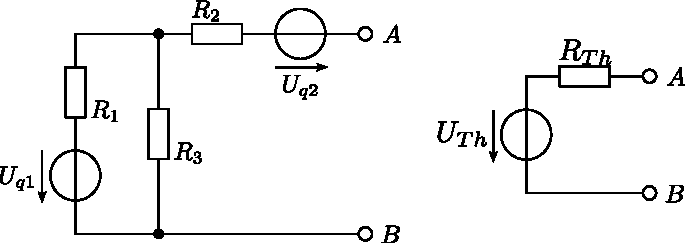
\includegraphics[scale=\schscale]{thevenin_sch_2.pdf}
\caption{Schaltung (l) und ihr Thévenin-Äquivalent (r)}
\label{sch:thevenin}
\end{figure}

\subsubsection{Berechnung}
\begin{itemize}
\item Leerlaufspannung $U_{Th}$ bestimmen (siehe Kapitel~\ref{sec:superpos})
\item Ersatzwiderstand ermitteln durch ausschalten aller unabhängiger Quellen (Spannungsquellen werden kurzgeschlossen, Stromquellen unterbrochen)
\end{itemize}

\newpage
\subsection{Norton-Theorem}
Nach Norton kann jedes Netzwerk bestehend aus Strom-, Spannungsquellen und Widerständen in eine Ersatzstromquelle\footnote{Norton-Äqivalent} gewandelt werden.

\begin{figure}[h!]
\centering
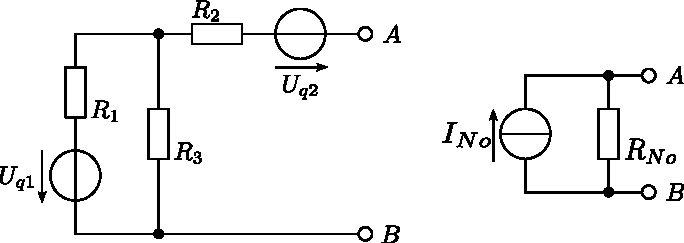
\includegraphics[scale=\schscale]{norton_sch_2.pdf}
\caption{Schaltung (l) und ihr Norton-Äquivalent (r)}
\label{sch:norton}
\end{figure}

\subsection{Spannungsquelle $\rightarrow$ Stromquelle}
\[ R_{No} = R_{Th} \]
\[ I_q = \frac{U_q}{R_{Th}} \]

\subsection{Stromquelle $\rightarrow$ Spannungsquelle}
\[ R_{Th} = R_{No} \]
\[ U_q = I_q \cdot R_{No} \]
